\documentclass{article}
\usepackage{amsmath,amsfonts,amsthm,amssymb,wasysym}
\usepackage{setspace}
\usepackage{enumitem}
\usepackage{Tabbing}
\usepackage{fancyhdr}
\usepackage{lastpage}
\usepackage{chngpage}
\usepackage{listings}
\usepackage{url}
\usepackage{subfigure}
\usepackage{array}
\usepackage{multicol}
\usepackage[color=blue!40]{todonotes}
\usepackage[protrusion=true,expansion,kerning]{microtype}
\usepackage{natbib}
\usepackage{capt-of}

% to adjust margins:
\topmargin=-0.25in
\evensidemargin=0in
\oddsidemargin=0in
\textwidth=6.25in
\textheight=8.5in
\headsep=0.25in

% homework specific information
\newcommand{\hmwkTitle}{CS645 Term Project}
\newcommand{\hmwkDueDate}{May 8, 2014}
\newcommand{\hmwkClass}{}
\newcommand{\hmwkClassInstructor}{}
\newcommand{\hmwkAuthorName}{Strubell, Verga}

% code listing settings
\lstset{
language=Python,                % choose the language of the code
basicstyle=\footnotesize\ttfamily,     % the size of the fonts that are used for the code
%numbers=left,                   % where to put the line-numbers
%numberstyle=\footnotesize,    % the size of the fonts that are used for the line-numbers
%stepnumber=2,                   % the step between two line-numbers.
%numbersep=5pt,                  % how far the line-numbers are from the code
showspaces=false,               % show spaces adding particular underscores
showstringspaces=false,         % underline spaces within strings
showtabs=false,                 % show tabs within strings adding particular underscores
frame=single,                   % adds a frame around the code
tabsize=2,                      % sets default tabsize to 2 spaces
captionpos=b,                   % sets the caption-position to bottom
breaklines=true,                % sets automatic line breaking
breakatwhitespace=false,        % sets if automatic breaks should only happen at whitespace
title=\ttfamily\lstname,     % show the filename of files included with \lstinputlisting;
frameround=fttt,
columns=fullflexible
}

% header and footer
\pagestyle{fancy}
\lhead{\hmwkAuthorName}
\chead{\hmwkTitle}
\rhead{\hmwkDueDate}   
\lfoot{}
\cfoot{}
\rfoot{\emph{Page\ \thepage\ of\ \pageref{LastPage}}}                          
\renewcommand\headrulewidth{0.4pt}
\renewcommand\footrulewidth{0.4pt}

\makeatletter
\newenvironment{tablehere}
  {\def\@captype{table}}
  {}

\newenvironment{figurehere}
  {\def\@captype{figure}}
  {}
\makeatother

%\renewcommand{\bibsection}{\subsubsection*{\refname}}

% Make title 
\title{
\LARGE\bf Datalog: A Logical Solution to the SIGMOD 2014 Programming Contest? \\
\date{}
\author{ Emma Strubell \and Patrick Verga}
}

\begin{document}

\maketitle

\begin{abstract}
For our term project we implemented two of the four SIGMOD 2014 programming contest queries each using two different Datalog query evaluation engines, comparing their query execution speed and memory footprint. The two Datalog engines that we compared were Iris \footnote{\protect\url{http://www.iris-reasoner.org/}}, the most prominent open-source Datalog engine, and SociaLite \cite{seo-et-al-13a}, a new Datalog system with extensions to support queries over web-scale social network graph data which is still in early beta and not yet open-source. We found that, although Iris performed better on the smaller dataset consisting of 1000 users, SociaLite vastly outperformed Iris on the larger dataset of 10,000 users, suggesting that although there is some startup overhead for small amounts of data in SociaLite's implementation, it scales much better than Iris for larger amounts of data. [MEMORY RESULTS]
\end{abstract}

\thispagestyle{fancy}

\begin{multicols}{2}

\section{Introduction}

For our class project we implemented a solution to two of the four queries making up the SIGMOD 2014 Programming Contest\footnote{\protect\url{http://www.cs.albany.edu/~sigmod14contest/task.html}} using two different Datalog engines. The aim of the contest was to perform some set of queries as quickly as possible. To do this, we had to create an efficient representation of the data as well as a mechanism for querying that data. The data for this year’s contest described the complex graph of interactions and entities making up a social network of 10,000+ individuals. Such social networks have become prevalent and bountiful sources of information that organizations can leverage to make useful predictions in many domains, given the computational tools for analyzing these graphs. Methods for efficiently synthesizing the information contained in these representations has become an important focus of research across the study of computer science, including that of database management systems.

As the rules of the contest dictated, our goal was to implement a system able to execute the contest queries as quickly as possible. Due to its lack of expressivity, SQL is not well suited for storing and querying recursive data structures such as graphs. The logical query language Datalog, which natively supports recursion, seems like a more natural solution to the problem of large-scale queries over graphs. However, previous research has found that existing ``vanilla'' Datalog implementations are still significantly slower than e.g. Java programs performing queries over graphically structured data due to a lack of flexibility provided to the user that is available in traditional programming languages \cite{seo-et-al-13a}. For example, existing Datalog engines insist that graphs be stored as relations despite the fact that adjacency lists are a significantly more efficient representation, and they do not provide mechanisms for the user to specify an evaluation order when a more efficient ordering might be known. Still, the advantages of a high-level, declarative database system such as Datalog over a general purpose programming language like Java are clear, one prominent benefit being automatic parallelization and optimization, but also of course ease of implementation. 

To address these shortcomings in existing Datalog implementations, Seo et al. \cite{seo-et-al-13a} describe a set of extensions to Datalog to facilitate efficient social network analysis called SociaLite\footnote{\protect\url{http://socialite-lang.github.io/}}, achieving performance within a few percentage points of highly optimized Java implementations of a number of graph algorithms, and greatly outperforming even commercial Datalog systems. They also have followed up on that original publication with additional extensions for using the MapReduce model in order to scale to even larger quantities of data \cite{seo-et-al-13b}. Unfortunately, the authors have not yet made their code open source (though they cited a mid-April date), but they did provide us with a compiled binary upon request. We implemented contest queries 2 and 3 using SociaLite as well as the open-source Datalog engine Iris\footnote{\protect\url{http://www.iris-reasoner.org/}} to evaluate (1) Datalog's proficiency in general at computing these types of queries and (2) the increase in query evaluation speed, if any, resulting from SociaLite's extensions to Datalog on the contest data. We found that, although Iris performed better on the smaller dataset consisting of 1000 users, SociaLite vastly outperformed Iris on the larger dataset of 10,000 users, suggesting that although there is some startup overhead for small amounts of data in SociaLite's implementation, it scales much better than Iris for larger amounts of data. We also compared memory footprints between the two implementations, finding Socialite to be much more memory efficient.

\section{Problem description}

This year’s SIGMOD contest posed four realistically complex queries over the given social network data. The contest provided two datasets simulating that of a large social network, generated by LDBC's social network benchmark generator\footnote{\protect\url{https://github.com/ldbc/ldbc_socialnet_bm}}, one ``small'' dataset made up of a network of 1000 individuals, and a ``large'' dataset of 10,000 users. The contest also evaluated entries on a ``huge'' dataset, but that data has not yet been made available. 

-- insert description of schema here

Due to time constraints and the overhead of performing a comparison between systems on top of implementing the queries themselves, we only implemented two of the four queries: Query 2 and Query 3. We also selected these queries because they were the two that could be performed the most within the constraints of the Iris system, which lacks recursive aggregate queries (required to compute shortest paths within a query).

The two queries we did not implement were Query 1 and Query 4. Query 1 asks for frequent communication paths of shortest distance in the graph. To perform this query, we need to find the shortest path between the two given individuals subject to some constraints over their communication metadata. Query 4, is to find the most central individuals in the network. In other words, we must find the people who are the most central or connected nodes (using the metric of betweenness centrality) in a subgraph derived by some constraints such as membership in a specific forum. As in Query 1, computing betweenness centrality also requires computing the shortest path between each pair of individuals in the graph. The second and third queries, which we implemented for this project, are described in more detail below.

\subsection{Query 2: Interests with Large Communities}
The goal of the second query is given some integer k and date d, to find the k interests with the largest underlying communities of users born on or after d.

To perform this query we required four tables: 
\begin{itemize}
\item person(id, birthday)
\item tag(tag.id, tagName)
\item person\_hasInterest\_tag(person.id, tag.id)
\item person\_knows\_person(person1.id, person2.id)
\end{itemize}

\subsection{Query 3: Socialization Suggestion}
The third query is to find closely connected pairs of people who are in the same location and share some number of interests, the goal being to recommend connections based on mutual interests. Given an integer k, integer h, and String p, find the k pairs of people who are associated with place p and are within h degrees of seperation with the most shared interests.

To perform this query we required ten tables: 
\begin{itemize}
\item place(id, name)
\item place\_isPartOf\_place(place1.id, place2.id)
\item person(id)
\item person\_hasInterest\_tag(person.id, tag.id)
\item person\_isLocatedIn\_place(person.id, place.id)
\item person\_workAt\_organisation(person.id, organisation.id)
\item person\_studyAt\_organisation(person.id, organisation.id)
\item person\_knows\_person(person1.id, person2.id)
\item organisation(id)
\item organisation\_isLocatedIn\_place(organisation.id, place.id)
\end{itemize}

\section{Datalog evaluation engines}

\subsection{Iris}

Iris (Integrated Rule Inference System) appears to be the most prominent (and well-documented) open source Datalog query evaluation engine, cited in \cite{seo-et-al-13a}, so we selected it as a baseline system to which to compare.

We wrote a java class implementing Iris' DataSource interface to read in the table .csv files and store the relevant columns. Because Iris lacks aggregate functions (recursive and non-recursive) the final aggregation steps of the query had to be implmented in java. 

\subsection{SociaLite}

The three main extensions in socialite are (1) tail-nested tables; (2) recursive aggregate functions; and (3) user-guided execution order. Tail nested tables address the issue of data representation, and allow for graph data to be represented efficiently as what are essentially adjacency lists rather than as traditional relations. Native support for certain recursive aggregate functions allows for common graph queries, such as those based on path length, to be expressed succinctly and to be evaluated efficiently using semi-naive evaluation. Finally, providing a mechanism for users to specify an evaluation order over vertices can significantly decrease the runtime required to traverse a graph if the graph is known to have a certain structure.

SociaLite is written in Java and takes input through a Jython wrapper. The user defines rules, facts, and queries either through an interactive interface or by providing a script which can be interleaved with python commands. Because we did not have access to the source code, we created code to generate query.py scripts which we submited to SociaLite. 


\section{Methods}

We implemented and evaluated Query 2 and Query 3 each on both the Iris and SociaLite query evalutation engines. All evaluation occurred in memory in both systems due to the limitations of the software packages, and rules were evaluated using semi-naive evaluation, which is the only strategy supported by Iris (in order to facilitate recursive aggregate functions). Both engines are implemented in Java, athough we were able to interact closely with the Java API in the case of Iris, we could only use SociaLite via its Python interface. In both cases we used Java to dynamically generate the queries given the inputs to the query (e.g. maximum number of hops) in each package's dialect of Datalog, which we then provided to the engine to evaluate. Any required post-processing was then performed in Java.

-- describe actual queries here
-- give example of each

Query 3 asks for the top k pairs of individuals connected by at most h hops who live, work or go to school in the same location, ranked by number of shared interests. We solved this problem by writing a function that generates a Datalog query given the inputs k, h and location. The following generated Datalog query provides an intermediate solution, lacking aggregation, to the contest query: query3(1, 2, ‘Amherst’):

\lstinputlisting{query3-example.py}

Query performed: \texttt{common\_interests(pid1,pid2,interest)}

The above produces all triples of people and interests that satisfy the location and hop constraints, including duplicates and self-pairs. We took this intermediary result and aggregated the top k counts of shared interests between non-duplicate pairs of users.																																												
\section{Results}
Queries were run on a machine with a 3.4 GhZ Intel Core i7 processor and 16GB RAM, which is comparable to that used for evaluating contest entries (8 CPU cores and 16GB RAM). All queries returned the correct results.
\begingroup
    \centering
    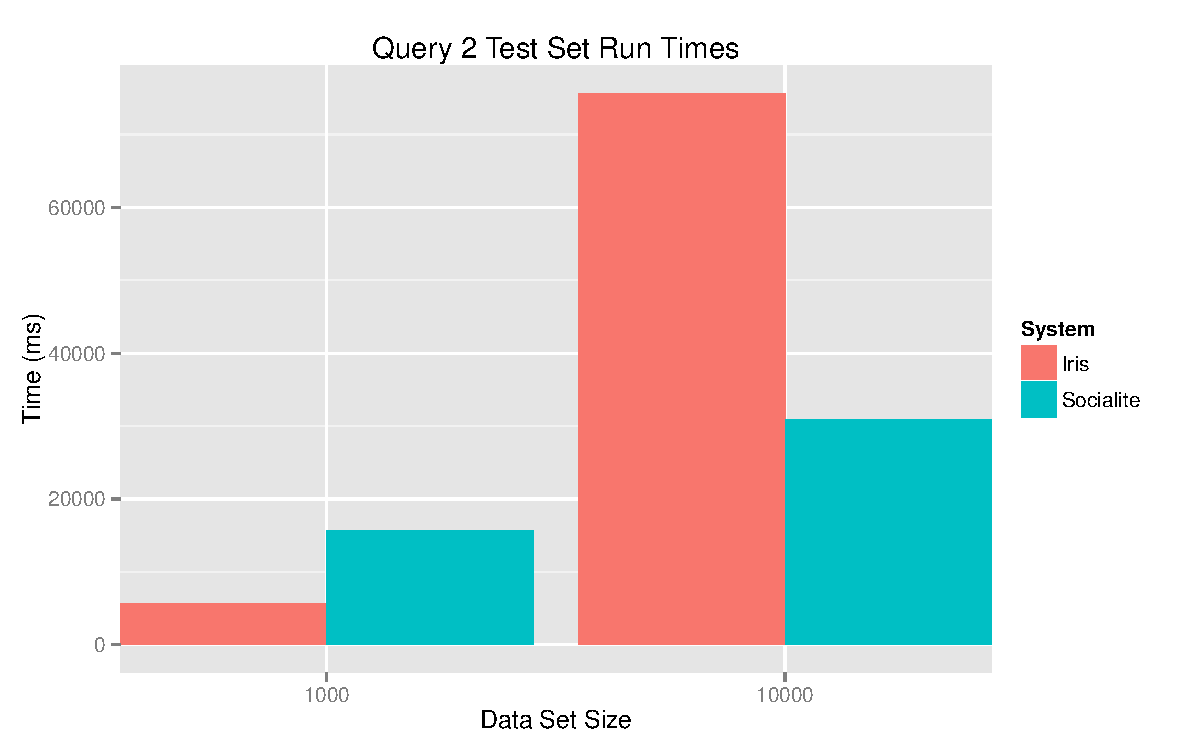
\includegraphics[scale=0.4]{../results/query2.pdf}
    \captionof{figure}{This is the caption}\label{fig:q2}
\endgroup

\begingroup
    \centering
    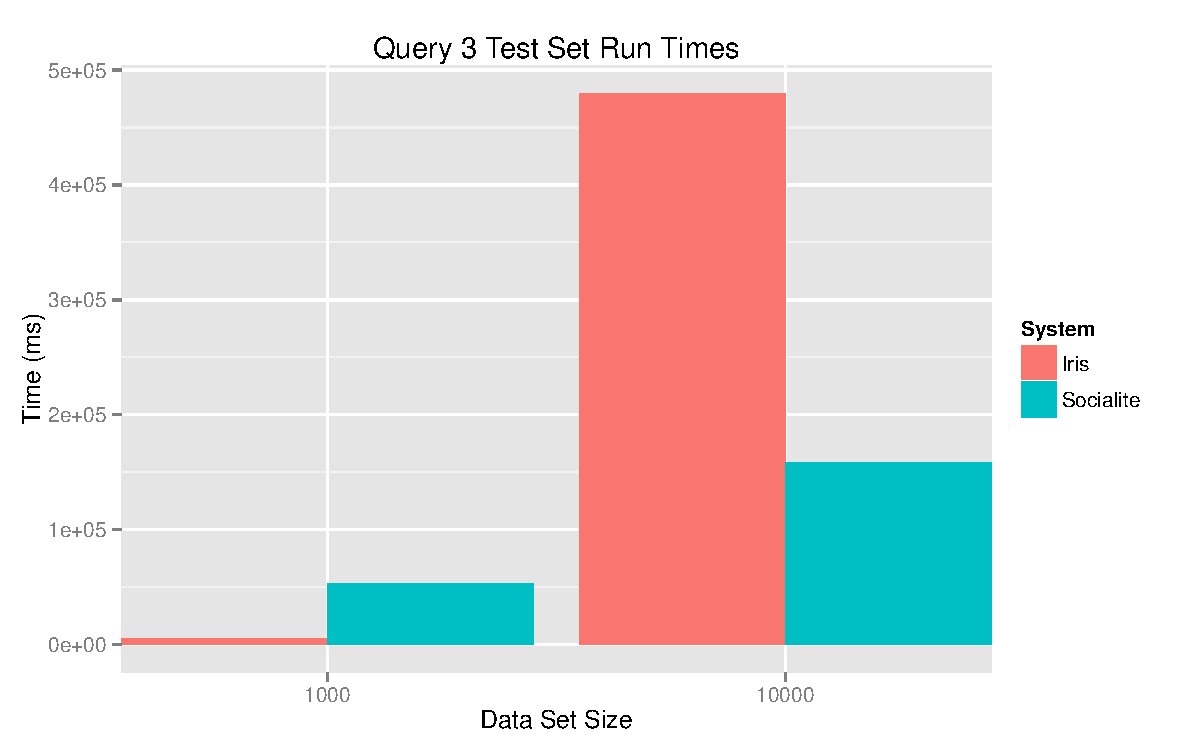
\includegraphics[scale=0.4]{../results/query3.pdf}
    \captionof{figure}{This is the caption}\label{fig:q3}
\endgroup

\begingroup
    \centering
    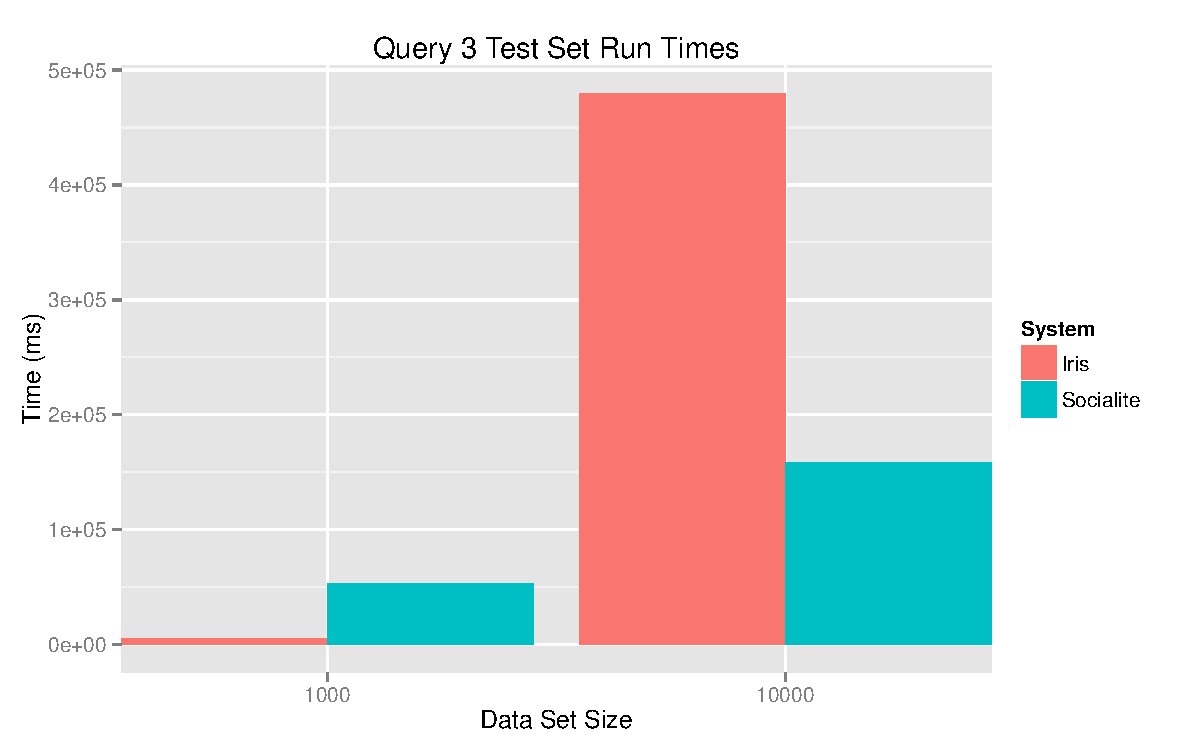
\includegraphics[scale=0.4]{../results/memory.pdf}
    \captionof{figure}{This is the caption}\label{fig:memory}
\endgroup
\section{Discussion}


\bibliography{cs645-project-report}
\bibliographystyle{unsrt}

\end{multicols}

\end{document}

%%% Local Variables: 
%%% mode: latex
%%% TeX-master: t
%%% End: 
